\section{Sezione Utente}
\label{sec:sezUtente}

\subsection{Impostazioni di sistema}
Nella sezione superiore destra dell'interfaccia, cliccando sull'icona impostazioni 
\includegraphics[height=1.2em]{assets/settings_icon.png} apparirà il menu laterale delle impostazioni di sistema.
\begin{figure}[H]
  \centering
  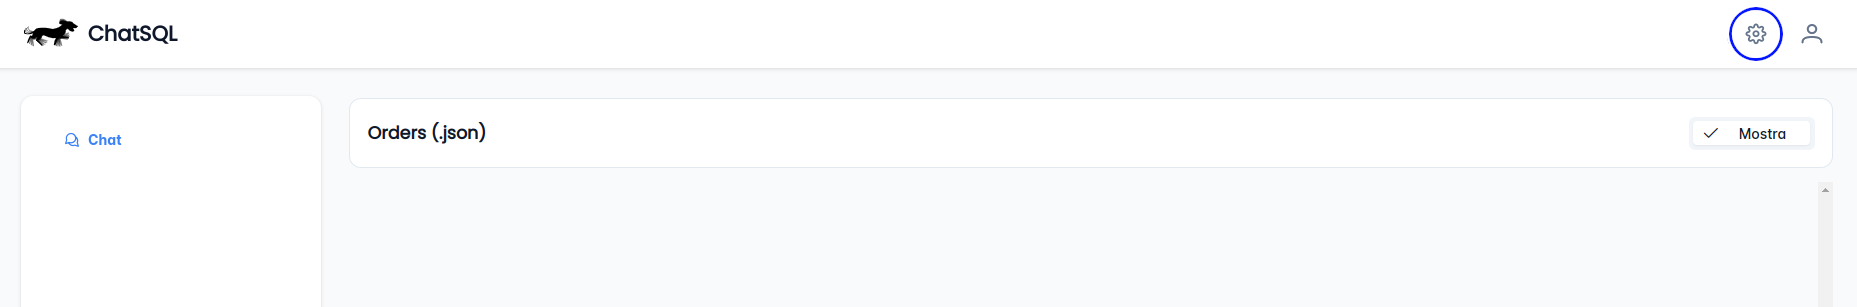
\includegraphics[width=1\textwidth]{assets/settings_topbar.png}
  \caption{Topbar con icona delle impostazioni}
\end{figure}
\begin{figure}[H]
  \centering
  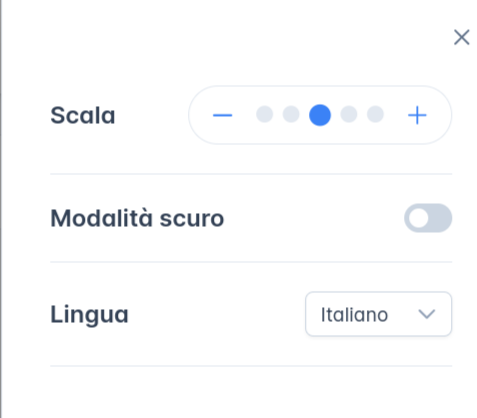
\includegraphics[width=0.50\textwidth]{assets/menu_config.png}
  \caption{Menu laterale delle impostazioni di sistema}
\end{figure}
\par Le impostazioni di sistema permettono di configurare le seguenti opzioni:
\begin{itemize}
  \item Scala: dimensioni del testo e della schermata; utile per adattare la dimensione dell'interfaccia alle proprie esigenze;
  \item Tema scuro: abilita o disabilita il tema scuro dell'interfaccia, per personalizzazione, accessibilità e comfort visivo;
  \item Lingua: selezione della lingua dell'interfaccia tra inglese e italiano (non cambia la lingua del \glossario{prompt} prodotto da ChatSQL, che rimane sempre in inglese).
\end{itemize}
\par Le modifiche apportate verranno memorizzate automaticamente, e applicate alla successiva apertura dell'applicazione.